\documentclass[tikz]{standalone}
\usepackage{pgfplots}
\pgfplotsset{/pgf/number format/use comma,compat=1.18}
\usepackage[T1]{fontenc}
\usepackage[utf8]{inputenc}
\usepackage{stanli} % TikZ Library for Structural Analysis by Jurgen Hackl
\usetikzlibrary{calc,intersections,patterns}
% frame definition, to be reused
\tikzset{ frame/.pic = {
    %points
	\point{A}{0}{3};
	\point{B}{3}{3};
	\point{C}{6}{3};
	\point{D}{9}{3};
	\point{E}{3}{0};
	\point{F}{6}{0};
	%beams
	\beam{2}{A}{B}[0][0];
	\beam{2}{B}{C}[0][0];
	\beam{2}{C}{D}[0][0];
	\beam{2}{E}{B}[0][0];
	\beam{2}{F}{C}[0][0];
	%supports
	\support{3}{A}[-90];
	\support{3}{D}[90];
	\support{3}{E}[0];
	\support{3}{F}[0];
	%node labels
	\notation{1}{A}{A}[below right];
	\notation{1}{B}{B}[below right];
	\notation{1}{C}{C}[below right];
	\notation{1}{D}{D}[below left];
	\notation{1}{E}{E}[above right];
	\notation{1}{F}{F}[above right];
	  }
	}

\begin{document}
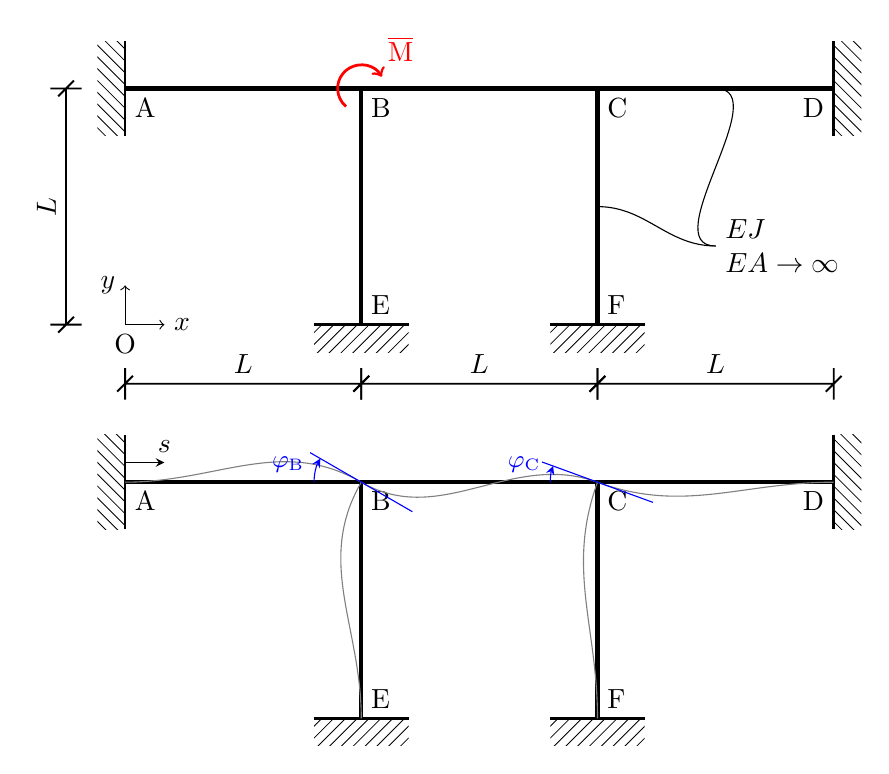
\begin{tikzpicture}[scale=1]
	%\draw [help lines] (0,0) grid [step=1] (9,3);
	% Coordinates system
	\draw(0,0)node[below]{O};
	\draw[<->] (0.5,0) node[right]{$x$}-|(0,0.5) node[left]{$y$};
	% the frame
	\pic at (0,0) {frame};
	% load force
	\begin{scope}[color=red]
		\load{2}{B}[30][200][0.3];
		\notation{1}{3.5,3.5}{$\overline{\mathrm{M}}$}[centered];
	\end{scope}
	% dimensions
	\dimensioning{2}{0,0}{A}{-0.75}[$L$];
	\dimensioning{1}{0,0}{E}{-0.75}[$L$];
	\dimensioning{1}{E}{F}{-0.75}[$L$];
	\dimensioning{1}{F}{9,0}{-0.75}[$L$];
	% other labels
	\draw(7.5,1)node[right,align=left]{$EJ$\\$EA\to\infty$} to [out=180,in=0] (6,1.5);
	\draw(7.5,1)node[right]{} to [out=180,in=0] (7.5,3);
	
	\begin{scope}[yshift=-5cm]
		% the frame
		\pic at (0,0) {frame};
		% deformation
		\draw [gray](A)to[out=0,in=150](B)to[out=-30,in=160](C)to[out=-20,in=180](D);
		\draw [gray](E)to[out=90,in=240](B);
		\draw [gray](F)to[out=90,in=250](C);
		% node rotations
		\draw [blue,rotate=-30]($(B)+(-0.75,0)$) -- ($(B)+(0.75,0)$);
		\draw [-stealth,blue](B) ++(180:6mm) node [above left] {\small$\varphi_\mathrm{B}$} arc (180:150:6mm); 
		\draw [blue,rotate=-20]($(C)+(-0.75,0)$) -- ($(C)+(0.75,0)$);
		\draw [-stealth,blue](C) ++(180:6mm) node [above left] {\small$\varphi_\mathrm{C}$} arc (180:160:6mm); 
		% local reference system
		\draw [|-stealth] (0,3.25) -- +(0.5,0) node [above] {$s$};
	\end{scope}
	
\end{tikzpicture}
\end{document}